\newcommand{\wormTagResultsAucTable}{
    \begin{table}[h!]
        \centering
        \begin{tabular}{|p{2,8cm}||P{2,2cm} P{2,2cm} P{2,2cm} P{2,2cm}|}
            \hline
            Worm Tag & ALOHA\newline (M/B only) & ALOHA & Joint\newline Embedding & Proposed\newline Model \\
            \hline
            AUC-ROC & - & \textBF{0.962$\pm$0.003} & 0.940$\pm$0.002 & 0.939$\pm$0.012 \\
            \hline
        \end{tabular}
        \caption[Worm Tag prediction task AUC-ROC results]{AUC-ROC (Area Under Curve) of the different models for the \textbf{Worm Tag} prediction task. Results were aggregated over \textBF{3} training runs with different weight initializations and minibatch orderings. Best results are shown in \textbf{bold}.} \label{tab:wormTag_auc}
    \end{table}
}

\newcommand{\wormTagResultsAtFprTable}{
    \begin{center}
        \begin{longtable}[c]{|P{3,2cm}||P{1,8cm} P{1,8cm} P{1,8cm} P{1,8cm} P{1,8cm}|}
            \hline
            Worm Tag & \multicolumn{5}{c|}{{FPR}} \\
            & $10^{-5}$ & $10^{-4}$ & $10^{-3}$ & $10^{-2}$ & $10^{-1}$ \\
            \hline
            \endfirsthead

            \caption*{\raggedright ...continued from previous page} \\
            \hline
            Worm Tag & \multicolumn{5}{c|}{\textbf{FPR}} \\
            & $10^{-5}$ & $10^{-4}$ & $10^{-3}$ & $10^{-2}$ & $10^{-1}$ \\
            \hline
            \endhead

            \caption*{\raggedleft ...continued on next page} \\
            \endfoot

            \caption[Worm Tag prediction task results]{Mean and standard deviation results (TPR, Accuracy, Recall, Precision and F1-Score) of the different models for the \textbf{Worm Tag} prediction task at different \textbf{FPR}s (\textit{False Positive Rates}). Results were aggregated over \textBF{3} training runs with different weight initializations and minibatch orderings. Best results are shown in \textbf{bold}. Under \textbf{TPR} results are also presented the percentage reduction in mean detection error and in ROC curve standard deviation introduced by the \textit{Proposed Model} with respect to both \textit{ALOHA} model and \textit{Joint Embedding}.} \label{tab:wormTag_results_at_fpr} \\
            \endlastfoot

            \multicolumn{6}{|c|}{\textbf{TPR}} \\
            \hline
            ALOHA (M/B only) & - & - & - & - & - \\
            ALOHA & 0.116$\pm$0.066 & 0.197$\pm$0.123 & 0.489$\pm$0.049 & \textBF{0.652$\pm$0.014} & \textBF{0.813$\pm$0.026} \\
            Joint Embedding & \textBF{0.145$\pm$0.002} & \textBF{0.288$\pm$0.061} & 0.518$\pm$0.047 & 0.647$\pm$0.017 & 0.770$\pm$0.014 \\
            Proposed Model & 0.112$\pm$0.074 & 0.175$\pm$0.107 & \textBF{0.559$\pm$0.033} & 0.641$\pm$0.021 & 0.786$\pm$0.031 \\
            \hline
            Error Reduction wrt\newline ALOHA (M/B only) & - & - & - & - & - \\
            Error Reduction wrt\newline ALOHA & -0.5\% & -2.7\% & 13.7\% & -3.2\% & -14.4\% \\
            Error Reduction wrt\newline Joint Embedding & -3.9\% & -15.9\% & 8.5\% & -1.7\% & 7.0\% \\
            \hline
            Std Reduction wrt\newline ALOHA (M/B only) & - & - & - & - & - \\
            Std Reduction wrt\newline ALOHA & -12.1\% & 13.0\% & 32.7\% & -50.0\% & -19.2\% \\
            Std Reduction wrt\newline Joint Embedding & -3600.0\% & -75.4\% & 29.8\% & -23.5\% & -121.4\% \\
            \hline
            \multicolumn{6}{|c|}{\textbf{Accuracy}} \\
            \hline
            ALOHA (M/B only) & - & - & - & - & - \\
            ALOHA & 0.860$\pm$0.010 & 0.873$\pm$0.019 & 0.918$\pm$0.008 & \textBF{0.936$\pm$0.002} & \textBF{0.886$\pm$0.004} \\
            Joint Embedding & \textBF{0.865$\pm$0.000} & \textBF{0.887$\pm$0.010} & 0.923$\pm$0.007 & 0.936$\pm$0.003 & 0.879$\pm$0.002 \\
            Proposed Model & 0.859$\pm$0.012 & 0.869$\pm$0.017 & \textBF{0.929$\pm$0.005} & 0.935$\pm$0.003 & 0.882$\pm$0.005 \\
            \hline
            \multicolumn{6}{|c|}{\textbf{Recall}} \\
            \hline
            ALOHA (M/B only) & - & - & - & - & - \\
            ALOHA & 0.116$\pm$0.066 & 0.197$\pm$0.123 & 0.489$\pm$0.049 & \textBF{0.652$\pm$0.014} & \textBF{0.813$\pm$0.026} \\
            Joint Embedding & \textBF{0.145$\pm$0.002} & \textBF{0.288$\pm$0.061} & 0.518$\pm$0.047 & 0.647$\pm$0.017 & 0.770$\pm$0.014 \\
            Proposed Model & 0.112$\pm$0.074 & 0.175$\pm$0.107 & \textBF{0.559$\pm$0.033} & 0.641$\pm$0.021 & 0.786$\pm$0.031 \\
            \hline
            \multicolumn{6}{|c|}{\textbf{Precision}} \\
            \hline
            ALOHA (M/B only) & - & - & - & - & - \\
            ALOHA & 0.999$\pm$0.000 & 0.996$\pm$0.002 & 0.989$\pm$0.001 & \textBF{0.925$\pm$0.002} & \textBF{0.605$\pm$0.008} \\
            Joint Embedding & \textBF{1.000$\pm$0.000} & \textBF{0.998$\pm$0.000} & 0.990$\pm$0.001 & 0.924$\pm$0.002 & 0.592$\pm$0.004 \\
            Proposed Model & 0.999$\pm$0.001 & 0.994$\pm$0.005 & \textBF{0.991$\pm$0.001} & 0.923$\pm$0.002 & 0.597$\pm$0.009 \\
            \hline
            \multicolumn{6}{|c|}{\textbf{F1 Score}} \\
            \hline
            ALOHA (M/B only) & - & - & - & - & - \\
            ALOHA & 0.202$\pm$0.102 & 0.313$\pm$0.162 & 0.653$\pm$0.045 & \textBF{0.764$\pm$0.010} & \textBF{0.694$\pm$0.014} \\
            Joint Embedding & \textBF{0.253$\pm$0.003} & \textBF{0.444$\pm$0.071} & 0.679$\pm$0.040 & 0.761$\pm$0.013 & 0.669$\pm$0.008 \\
            Proposed Model & 0.194$\pm$0.119 & 0.283$\pm$0.159 & \textBF{0.714$\pm$0.027} & 0.757$\pm$0.016 & 0.678$\pm$0.018 \\
            \hline
        \end{longtable}
    \end{center}
}

\newcommand{\wormTagResultsSummaryTable}{
    \begin{table}[h!]
        \centering
        \begin{tabular}{|P{3,2cm}||P{1,8cm} P{1,8cm} P{1,8cm} P{1,8cm} P{1,8cm}|}
            \hline
            \multicolumn{6}{|c|}{Worm Tag (at FPR $=1\%$)} \\
            \hline
            Model & TPR & Accuracy & Precision & Recall & F1 score \\
            \hline
            ALOHA (M/B only) & - & - & - & - & - \\
            ALOHA & \textBF{0.652$\pm$0.014} & \textBF{0.936$\pm$0.002} & \textBF{0.925$\pm$0.002} & \textBF{0.652$\pm$0.014} & \textBF{0.764$\pm$0.010} \\
            Joint Embedding & 0.647$\pm$0.017 & 0.936$\pm$0.003 & 0.924$\pm$0.002 & 0.647$\pm$0.017 & 0.761$\pm$0.013 \\
            Proposed Model & 0.641$\pm$0.021 & 0.935$\pm$0.003 & 0.923$\pm$0.002 & 0.641$\pm$0.021 & 0.757$\pm$0.016 \\
            \hline
        \end{tabular}
        \caption[Summary of Worm Tag prediction task results]{Summary of the mean and standard deviation results of the different models for the \textbf{Worm Tag} prediction task at \textbf{FPR} $=1\%$. Results were aggregated over \textBF{3} training runs with different weight initializations and minibatch orderings. Best results are shown in \textbf{bold}.} \label{tab:wormTag_result_summary}
    \end{table}
}

\newcommand{\wormTagRocAlohaMB}{
    \begin{figure}[h!]
        \vspace*{-0.5cm}
        \centering
        \includegraphics[width=0.6\textwidth]{./results/worm_tag_roc_alohaMB.png}
        \vspace*{-0.2cm}
        \caption[Worm Tag prediction task ALOHA (M/B only) ROC curve]{ROC curve and AUC statistics of \textBF{ALOHA (M/B only)} model for the \textbf{Worm Tag}. The line represents the \textit{mean} TPR at a given FPR, while the shaded region represents the \textit{standard deviation}. Statistics were computed over \textBF{3} training runs, each with random parameter initialization.}
        \label{fig:wormTagRocAlohaMB}
    \end{figure}
}

\newcommand{\wormTagRocAloha}{
    \begin{figure}[h!]
        \vspace*{-0.5cm}
        \centering
        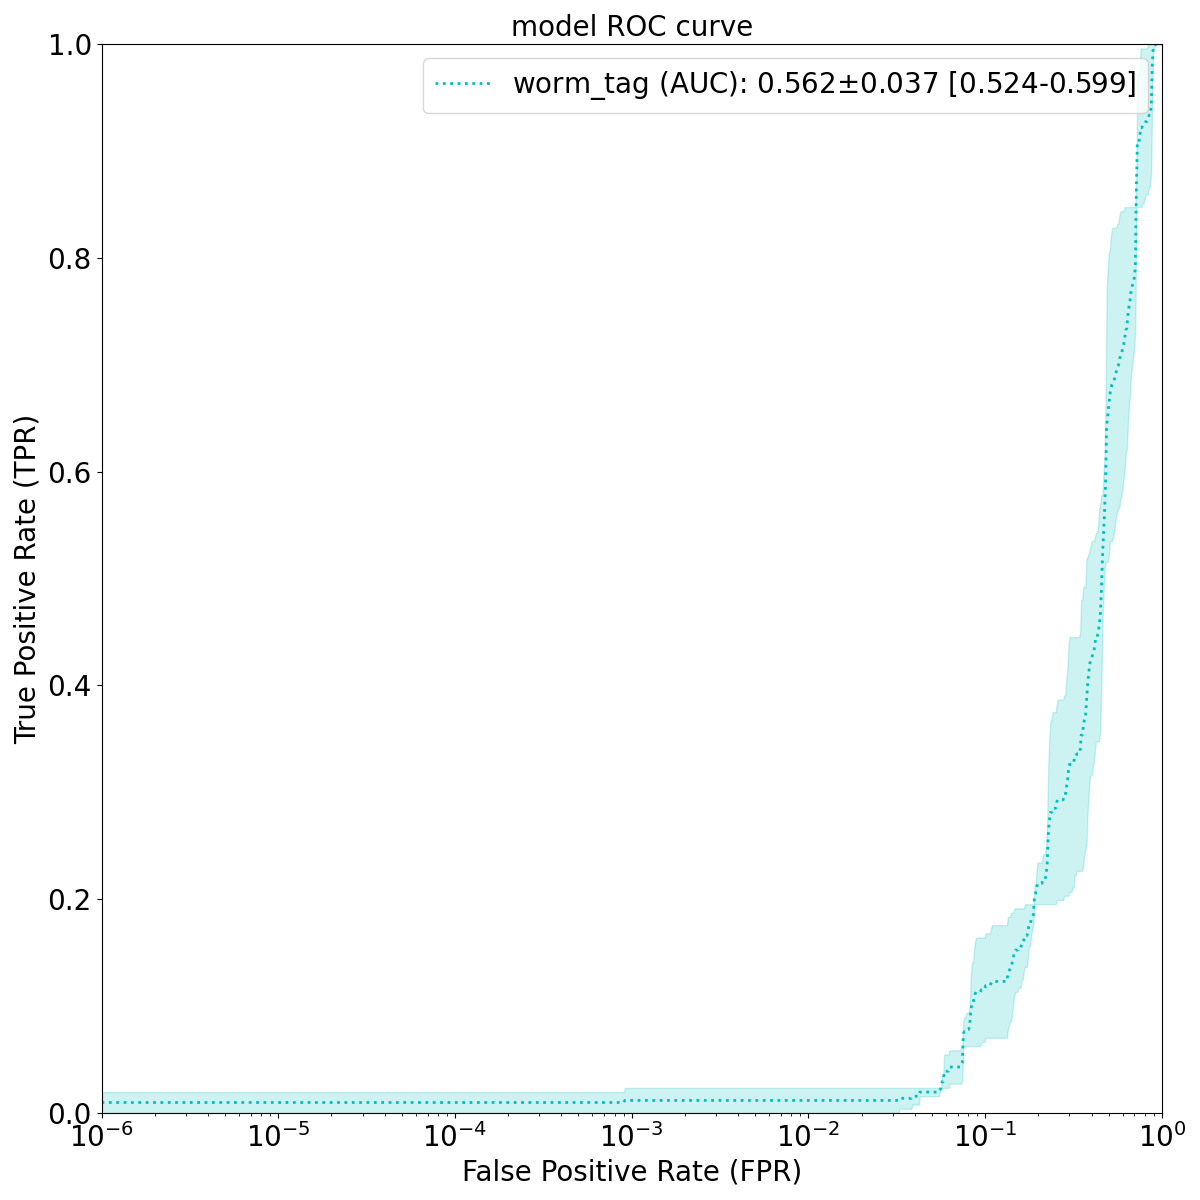
\includegraphics[width=0.6\textwidth]{./results/worm_tag_roc_aloha.png}
        \vspace*{-0.2cm}
        \caption[Worm Tag prediction task ALOHA ROC curve]{ROC curve and AUC statistics of \textBF{ALOHA} model for the \textbf{Worm Tag}. The line represents the \textit{mean} TPR at a given FPR, while the shaded region represents the \textit{standard deviation}. Statistics were computed over \textBF{3} training runs, each with random parameter initialization.}
        \label{fig:wormTagRocAloha}
    \end{figure}
}

\newcommand{\wormTagRocJointEmbedding}{
    \begin{figure}[h!]
        \vspace*{-0.5cm}
        \centering
        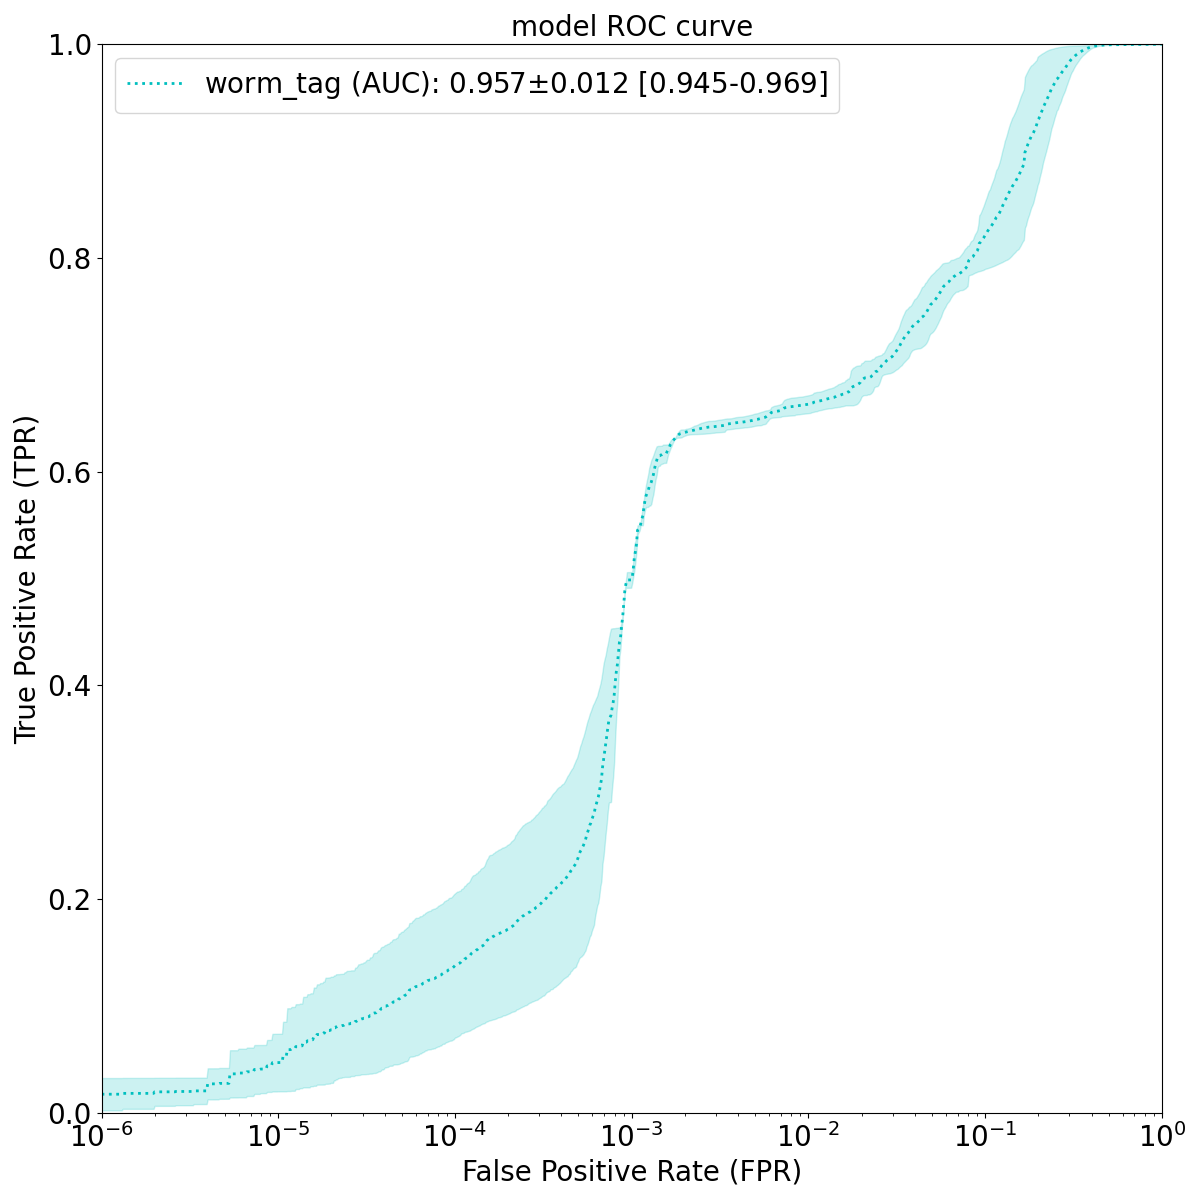
\includegraphics[width=0.6\textwidth]{./results/worm_tag_roc_jointEmbedding.png}
        \vspace*{-0.2cm}
        \caption[Worm Tag prediction task Joint Embedding ROC curve]{ROC curve and AUC statistics of \textBF{Joint Embedding} model for the \textbf{Worm Tag}. The line represents the \textit{mean} TPR at a given FPR, while the shaded region represents the \textit{standard deviation}. Statistics were computed over \textBF{3} training runs, each with random parameter initialization.}
        \label{fig:wormTagRocJointEmbedding}
    \end{figure}
}

\newcommand{\wormTagRocProposedMethod}{
    \begin{figure}[h!]
        \vspace*{-0.5cm}
        \centering
        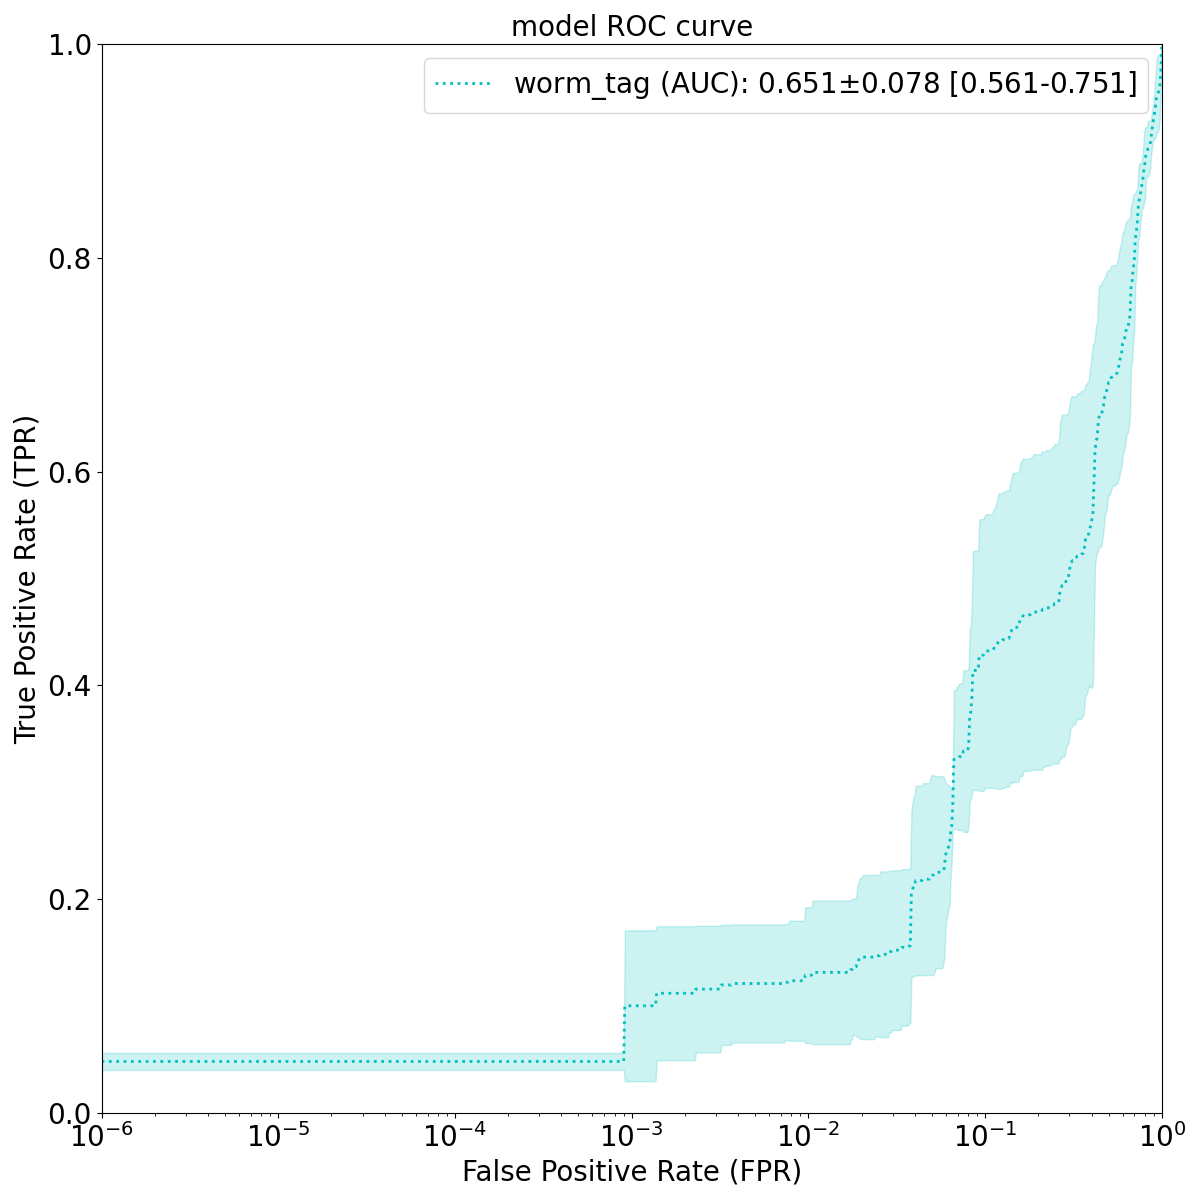
\includegraphics[width=0.6\textwidth]{./results/worm_tag_roc_proposedModel.png}
        \vspace*{-0.2cm}
        \caption[Worm Tag prediction task Proposed Model ROC curve]{ROC curve and AUC statistics of \textBF{Proposed Model} for the \textbf{Worm Tag}. The line represents the \textit{mean} TPR at a given FPR, while the shaded region represents the \textit{standard deviation}. Statistics were computed over \textBF{3} training runs, each with random parameter initialization.}
        \label{fig:wormTagRocProposedModel}
    \end{figure}
}
